\documentclass[11pt]{article}
\usepackage[T1]{fontenc}
\usepackage{lmodern}
\usepackage{amssymb, amsmath, amsthm}
\usepackage{mathtools}
\usepackage{graphicx}
\usepackage[colorlinks=true, linkcolor=blue, citecolor=blue, urlcolor=blue]{hyperref}
\usepackage{lipsum}
\usepackage{comment}
\usepackage{enumitem}
\usepackage{tikz-cd}
\usepackage{tikz}
\usetikzlibrary{shapes,arrows,positioning,shadows}
\usepackage[margin=1in]{geometry}
\usepackage{xcolor}
\definecolor{plum}{RGB}{221,160,221} % used by the cost-matrix figure
\usepackage{algorithm}
\usepackage[noend]{algorithmic}
% NOTE: algpseudocode is intentionally not loaded: it conflicts with
% algorithmic, and the pseudocode below uses algorithmic commands.
\usepackage{caption}
\usepackage{etoolbox} % for \ifblank in myalgorithm

\usepackage{verbatim}

\newenvironment{myalgorithm}[1][]{%
  \par\vspace{8pt}
  \noindent\hrule height.8pt
  \vspace{4pt}
  \ifblank{#1}{}{%
    \captionof{algorithm}{#1}%
    \vspace{4pt}
    \noindent\hrule height.4pt
    \vspace{6pt}
  }%
}{%
  \vspace{6pt}
  \noindent\hrule height.8pt
  \par\vspace{8pt}
}

% Custom packages
\usepackage{flexart}
\usepackage[many]{tcolorbox} %box environment
\usepackage[normalem]{ulem} %custom underline

% Bar width and spacing
\newlength{\framelinewidth}
\setlength{\framelinewidth}{0.6mm}
\newlength{\marginsep}
\setlength{\marginsep}{3pt}
\newlength{\defparindent}
\setlength{\defparindent}{15pt}
\setlength{\parindent}{\defparindent}
\newlength{\boxparskip}
\setlength{\boxparskip}{\parskip}

%Define colors
% https://davidmathlogic.com/colorblind/#%23038DFC-%232B65C6-%2322AA22-%23003300
\definecolor{aicolor}{HTML}{038DFC} 
\definecolor{editedaicolor}{HTML}{2B65C6}
\definecolor{humancolor}{HTML}{22AA22}  
\definecolor{aiassistedcolor}{HTML}{003300}
\definecolor{defaultcolback}{HTML}{FFFFFF}  % white
\newcommand{\opacityFrame}{0.5} %Opacity Percentage for the Frame
\newcommand{\opacityText}{0.7} %Opacity Percentage for the Label Text

%Define footenote commands: Creates an aux file for the footnotes inside the boxes
\newif\iffootaux
\newcounter{footaux}% for \csname
\newcounter{auxpage}% to handle frontmatter etc.
\setcounter{auxpage}{1}

\makeatletter

\def\tcb@footnote@setup{
\let\footnotetext=\footaux
\let\footnote=\footnoteaux
}
  
\def\footnoteaux{\@ifnextchar[\@xfootnoteaux{\stepcounter{footnote}%
  \footnotemark[\thefootnote]\@footaux[\thefootnote]}}
  
\def\@xfootnoteaux[#1]{\footnotemark[#1]\@footaux[#1]}

\def\footaux{\@ifnextchar[\@footaux{\@footaux[\thefootnote]}}
\def\@footaux[#1]#2{\protected@write{\@auxout}{\let\theauxpage\relax}{\string\newfootnote{\theauxpage}{#1}{#2}}}

\newcommand{\newfootnote}[3]{% #1 = \theauxpage, #2 = \thefoontnote, #3 = text
  \ifnum#1=1\relax
    \footnotetext[#2]{#3}%
  \else
    \stepcounter{footaux}%
    \expandafter\xdef\csname footauxpage\thefootaux\endcsname{#1}%
    \expandafter\xdef\csname footauxnumber\thefootaux\endcsname{#2}%
    \expandafter\protected@xdef\csname footauxtext\thefootaux\endcsname{#3}%
  \fi}

% to run at the end of every page (debug version)
\newcommand{\addfootaux}{\loop
  \@ifundefined{footauxpage\thefootaux}{\footauxfalse}{%
    \count1=\csname footauxpage\thefootaux\endcsname\relax
    \advance\count1 by -1
    \ifnum\count1=\value{auxpage}%
      \expandafter\let\expandafter\footauxnumber\csname footauxnumber\thefootaux\endcsname
      \expandafter\let\expandafter\footauxtext\csname footauxtext\thefootaux\endcsname
      \footnotetext[\footauxnumber]{\footauxtext}%
      \footauxtrue
    \else
      \footauxfalse
    \fi}
  \iffootaux
    \global\expandafter\let\csname footauxpage\thefootaux\endcsname\relax
    \global\expandafter\let\csname footauxnumber\thefootaux\endcsname\relax
    \global\expandafter\let\csname footauxtext\thefootaux\endcsname\relax
    \stepcounter{footaux}%
  \repeat
\stepcounter{auxpage}}
\makeatother

\AtBeginDocument{\setcounter{footaux}{1}}% reset counter after \newfootnote
\AddToHook{shipout/after}{\addfootaux}


%Define box styles
\makeatletter
\tcbset{
    roundbox/.style={
    % Box Options
    rounded corners,
    arc=3mm,
    boxrule=\framelinewidth
  },
  rectanglebox/.style={
    % Box Options
    sharp corners,  
    boxrule=\framelinewidth
  },
    linemargin/.style={
    % Box Options
    % Make frame with 1 line
    sharp corners,   
    leftrule=\framelinewidth,    % Thickness of the left line
    rightrule=-0.1mm,            % Removes right frame
    toprule=-0.1mm,              % Removes top frame
    bottomrule=-0.125mm,         % Removes bottom frame
    % % make white background
    colback=white,  
    % Oversize makes bigger, so that text alings with rest of the document
    oversize,
    % box margins 
    left=\marginsep,                                
    right=\marginsep,
    top=0.5pt,
    bottom=0.5pt,
    before skip=0.5\baselineskip,
    after skip=0.5\baselineskip
  },
  alignoptions/.style={
    % box margins 
    left=\marginsep, 
    right=\marginsep,
    top=0.5pt,
    bottom=0.5pt,
    before skip=0.5\baselineskip,
    after skip=\parskip,
    before upper={
    \parindent=\defparindent
    \setlength{\parskip}{\boxparskip}
    }
  },
  %Format for footnotes to appear in the correct page
  footnoteformat/.style={
  before upper app=\tcb@footnote@setup
  }
}
\makeatother

\tcbset{
  enhancebreak/.style={
    % Box Options
    enhanced,
    breakable,    
    skin first=enhanced,
    skin middle=enhanced,
    skin last=enhanced,
    % Oversize makes bigger, so that text alings with rest of the document
    oversize,
  },
}

% Define Tcolorbox environments
%% Args: #1 additional options, #2 color, #3 Side text label
\newtcolorbox{labeledblock}[3][]{
    colframe=#2,opacityframe=\opacityFrame,
    enhancebreak, alignoptions, linemargin, 
    colback=white,
    overlay={
    \node[
    #2, font=\tiny\bfseries\sffamily, 
    rotate=90, anchor=east, align=right,
    text opacity=\opacityText
      ]
      at ([xshift=-\marginsep-\framelinewidth/2, yshift=3pt]frame.north west) {#3};
    }, footnoteformat,
    #1
}

\newtcolorbox{humanblock}[1][]{
    colframe=humancolor, opacityframe=\opacityFrame,
    enhancebreak, alignoptions, linemargin,
    colback=white,
    overlay={
    \node[
    humancolor, font=\tiny\bfseries\sffamily, 
    rotate=90, anchor=east, align=right, 
    text opacity=\opacityText
      ]
      at ([xshift=-\marginsep-\framelinewidth/2, yshift=3pt]frame.north west) {Human};
    }, footnoteformat,
    #1
}

\newtcolorbox{aiassistedblock}[1][]{
    colframe=aiassistedcolor, opacityframe=\opacityFrame,
    enhancebreak, alignoptions, linemargin,
    colback=white,
    overlay={
    \node[aiassistedcolor, font=\tiny\bfseries\sffamily, rotate=90, anchor=east, align=right,
      text opacity=\opacityText
      ]
      at ([
      xshift=-\marginsep-\framelinewidth/2-4pt, yshift=3pt
      ]frame.north west) {Human: \\ AI-assisted};
    }, footnoteformat,
    #1
}

\newtcolorbox{aiblock}[1][]{
    colframe=aicolor, opacityframe=\opacityFrame,
    enhancebreak, alignoptions, linemargin, 
    colback=white,
    overlay={
    \node[aicolor, font=\tiny\bfseries\sffamily, rotate=90, anchor=east, align=right,
      text opacity=\opacityText
      ]
      at ([xshift=-\marginsep-\framelinewidth/2, yshift=3pt]frame.north west) {AI};
    }, footnoteformat,
    #1
}

\newtcolorbox{editedaiblock}[1][]{
    colframe=editedaicolor, opacityframe=\opacityFrame,
    enhancebreak, alignoptions, linemargin,
    colback=white,
    overlay={
    \node[
    editedaicolor, font=\tiny\bfseries\sffamily, 
    rotate=90, anchor=east, align=right, 
    text opacity=\opacityText
      ]
      at ([xshift=-\marginsep-\framelinewidth/2, yshift=3pt]frame.north west) {Edited AI};
    }, footnoteformat,
    #1
}


%%%---------------------- Underline Commands -------------------------

% Dash pattern:
\gdef\dashpattern{\kern.05em\lower.3ex\vbox{\hrule width.2em\kern.1ex}}

\def\humanul{\textcolor{humancolor}\bgroup\markoverwith{\kern.05em\lower.3ex\vbox{\hrule width.2em\kern.1ex}\kern.05em}\ULon}

\def\aiul{\textcolor{aicolor}\bgroup\markoverwith{\kern.05em\lower.3ex\vbox{\hrule width.2em\kern.1ex}\kern.05em}\ULon}
\newcommand{\Muse}{
% \footnotesize with
{Muse Spark} via {\ttfamily \href{http://meta.ai}{meta.ai}}}
\newcommand{\HumanLabel}{
({\bfseries\sffamily\color{humancolor!70}Human})
}
\newcommand{\AILabel}{
({\bfseries\sffamily\color{aicolor!70}AI})
}

% \sq{row}{col}{symbol}: one labeled square, rows/cols numbered from 1.
% Cells are 0.5cm; font size is unaffected (node text never scales).
\newcommand{\sq}[3]{%
  \draw ({(#2-1)*0.5},{-(#1-1)*0.5}) rectangle ++(0.5,-0.5);
  \node at ({(#2-0.5)*0.5},{-(#1-0.5)*0.5}) {#3};%
}

\newcommand{\cR}{\mathcal R}
\newcommand{\cB}{\mathcal B}
\newcommand{\nil}{\textsf{nil}}

%GAP Code boxes
\definecolor{codebg}{RGB}{245,245,245}
\usepackage{listings}
%
\lstdefinelanguage{GAP}{
  morekeywords={if,then,else,elif,fi,for,do,od,while,local,function,return,rec,Error},
  sensitive=true,
  morecomment=[l]{\#},
  morestring=[b]",
  morestring=[b]'
}
\lstset{
  language=GAP,
  basicstyle=\footnotesize\ttfamily,
  keywordstyle=\color{blue}\bfseries, % <- blue differentiators
  commentstyle=\color{gray}\itshape,
  stringstyle=\color{red!60!black},
  backgroundcolor=\color{codebg},
  frame=single,
  framerule=0.4pt,
  rulecolor=\color{black!5},
  breaklines=true,
  columns=fullflexible,
  keepspaces=true,
  upquote=true,
  showstringspaces=false
}


%% Commands
%%%_____________________________________


\newtheorem{thm}{Theorem}[section]
\newtheorem{cor}[thm]{Corollary}
\newtheorem{lem}[thm]{Lemma}
\newtheorem{prop}[thm]{Proposition}
\newtheorem{con}[thm]{Conjecture}

\theoremstyle{definition}
\newtheorem{defn}[thm]{Definition}
\newtheorem{qst}[thm]{Question}
\newtheorem{assumption}[thm]{Assumption}
\newtheorem{rem}[thm]{Remark}
\newtheorem{exm}[thm]{Example}

\numberwithin{equation}{section}


\font\com=cmtt10
\def\hb{\hfill\break}
\def\comment#1{\hb {\com\par\hskip2in \#\#\#\#\#\#\par #1 \par\hskip2in
\#\#\#\#\#\#}\hb}



%% short title (plain article's \title takes no optional argument)
\title{From Log-Cubed to Log in Bichromatic Sorting}
% \subtitle{Every key group exercised in one document}
%% Declare each note once, then mark as many authors as you like with it.

% \newfanote{orch}{Orchestrating author}
% \newfanote{supp}{Supporting author}
\newfanote{rev}{Reviewing author}

\primaryauthors{
{\scshape \Muse}
}

\newcommand{\secondaryAuthorsLabel}{Reviewed by}

\secondaryauthors{
{\scshape Tyler Foster}\fanote{rev} % reviewing author
}
%\normalfont \scshape
\flexset{
titlefont = \large
\bfseries
\spaceskip1.3
\fontdimen2\font
plus1.3
\fontdimen3\font
\relax,
secondarylabel = {\secondaryAuthorsLabel},
thmplainabove = 0.6em,
thmdefinitionabove = 0.6em,
thmplainbelow = 0em,
thmdefinitionbelow = 0em,
proofabove = 0em,
}

\subjclass[2020]{68P10, 68W20}
% \affiliation{Department of Typographic Engineering, Example University}
% \keywords{bichromatic sorting, priced comparisons, randomized algorithms}
\flexabstract{%
We give a randomized algorithm for sorting red and blue elements when
mixed comparisons cost $1$ and monochromatic comparisons cost
$\alpha > 1$ and $\beta > 1$. Writing $H$ for the cost of the
adjacent pairs in the sorted order, the algorithm sorts with expected
cost $O(H \log N)$, improving the $O(H \log^3 N)$ bound of Goswami
and Jacob to the optimal logarithmic competitive ratio. The algorithm
inserts red elements in random order into alternating runs located
by binary search on representatives, and charges its work to records
in the insertion order.
We remark on the use of AI in this research, see Statement of AI Use.
}

\begin{document}

\maketitle

\begin{section}{Introduction}
\begin{humanblock}
\begin{subsection}{Sorting by comparison, with colors}
{\em Sorting} is the computational task that takes
    \begin{itemize}[label=$\bullet$]
    \item {\em Input}: finite sequence $X$ of distinct elements with $\mathbb{Z}_{>0}$-valued keys,
    \end{itemize}
and returns
    \begin{itemize}[label=$\bullet$]
    \item {\em Output}: original sequence rearranged so that keys are now in order.
    \end{itemize}
The basic unit of verification for any sorting algorithm is the pairwise comparison that decides, for a given pair of distinct $x\neq x'$ in $X$, if
$$
\text{key}(x)\;>\;\text{key}(x')\quad\quad\text{or}\quad\quad\text{key}(x)\;<\;\text{key}(x').
$$
Each such comparison incurs a computational cost $\operatorname{cost}(x,x')>0$ that depends on the pair of elements being compared, and one of the standard ways of measuring the efficiency of a given sorting algorithm is by computing its {\em total cost}, meaning the sum of the costs of all comparisons made over the course of a given run of the algorithm.

When the costs of comparisons do {\em not} depend on the specific elements being compared, i.e., when comparison costs are constant, we can normalize so that all costs are equal to $1$. In this case, an optimal algorithm, {\ttfamily MergeSort}, sorts $N$ elements by comparisons with tight asymptotic bound on total cost of $\Theta(N \log N)$ comparisons, where $N:=\#X$ denotes the number of elements in $X$, and where $\log$ denotes the logarithm to base $2$~\cite{knuth1998art}. In particular, the cost is
$$
O(N\cdot\operatorname{log}\,N).
$$

When comparison costs are {\em not} constant across all pairs of elements in $X$, we face a potential explosion in possibilities, since there are $\frac{N^2-N}{2}$ distinct pairs of elements in $X$, where again $N$ denotes the number of elements in $X$. To make asymptotic statements, we have to consider natural families whose comparison costs have some kind of stable structure.

One natural such family supposes that the elements of our original sequence $X$ fall into two types, sometimes called {\em nuts} and {\em bolts} and sometimes called {\em red} and {\em blue}, such that comparisons between pairs of red elements have some fixed cost $\alpha>0$, comparisons between pairs of blue elements have fixed cost $\beta>0$, and comparisons between red and blue elements have fixed cost $\gamma$. In this case, we denote the subsets of red and blue elements in $X$ by $\mathcal{R}$ and $\mathcal{B}$, respectively, so that as a set, $X$ is a disjoint union
$$
X\;=\;\mathcal{R}\sqcup\mathcal{B}
$$
If we normalize by dividing all comparison costs by $\gamma$ in this case, we get the {\em comparison cost upper-triangular block matrix}
$$
\begin{array}{c}
\ \ \ \ \ 
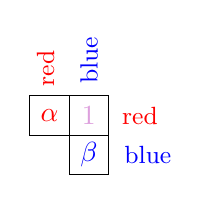
\begin{tikzpicture}
  \sq{1}{1}{{\color{red} $\alpha$}}  \sq{1}{2}{{\color{plum} $1$}}
                       \sq{2}{2}{{\color{blue} $\beta$}}
  % column colors, reading horizontally on top
  \node[rotate=90] at (0.2,0.35) {{\color{red}\small red}};
  \node[rotate=90] at (0.75,0.45) {{\color{blue}\small blue}};
  % row colors, on the right
  \node at (1.4,-0.25) {{\color{red}\small red}};
  \node at (1.5,-0.75) {{\color{blue}\small blue}};
\end{tikzpicture}\\
\text{comparison cost matrix}
\end{array}
$$

When $\alpha<1$ or $\beta<1$, then monochromatic comparisons are the
cheap ones, and the natural strategy sorts each color class
internally --- at $O(\alpha N \log N)$ and $O(\beta N \log N)$ --- before merging the two sorted lists with $O(N)$ mixed comparisons.

Throughout, the {\em competitive ratio} of an algorithm for this problem is the worst case, over all inputs, of its total comparison cost --- its expected total cost, for a randomized algorithm --- divided by the benchmark $H$ of the input, defined next; in the priced-information framework of Charikar et al.~\cite{charikar2000query}, $H$ is the cost of the cheapest proof that the output is sorted.

Thus we assume that $\alpha,\beta>1$. In this case, Goswami and Jacob~\cite{goswami2024bichromatic} construct a randomized algorithm, {\ttfamily InversionSort}, with competitive ratio $O(\log^3 N)$ with high probability, and they conjecture that the optimal $O(\log N)$ ratio is achievable. Given any {\em ordered} sequence of red and blue elements, we define its {\em benchmark} to be the sum of the costs required to compare adjacent pairs of keys in the sequence. In other words, it is the cost required to verify that the sequence is indeed in order. For an arbitrary, not necessarily ordered sequence, we define its benchmark to be the benchmark of its ordered counterpart. Goswami and Jacob refer to $H$ as the {\em Hamiltonian of the cost}, and they prove that the expected cost of {\ttfamily InversionSort} is
$$
O(H \log^3 N).
$$
Goswami and Jacob's conjectured competitive ratio $O(\log N)$ would bring this expected cost down to $O(H \log N)$.

In the present paper, we introduce a new randomized bichromatic sorting algorithm called {\em SpliceSort}, developed with Muse Spark via {\ttfamily \href{http://meta.ai}{meta.ai}}, and we prove that its expected cost is
$$
O(H\cdot\operatorname{log}\,N).
$$
This is optimal up to the logarithmic factor, since $H$ is itself a lower bound on the cost of any comparison algorithm (Proposition~\ref{prop:Hlower}), and the $\Omega(\log N)$ lower bound on the competitive ratio carries over from unit-cost sorting~\cite{goswami2024bichromatic}. This provides a substantial improvement over {\ttfamily InversionSort}, whose exponent is $3$ where ours is $1$.

\end{subsection}

% \medskip
% \medskip

\begin{thm}\label{thm:main}
There exists a randomized comparison algorithm that sorts every
bichromatic input of size $N$ with monochromatic costs
$\alpha, \beta > 1$ and whose expected total comparison cost is
$O(H \log N)$, where $H$ is the cost of comparing adjacent pairs in the
sorted order, i.e., the cost of verifying that the final sequence is ordered. The implicit constant is absolute.
\end{thm}

\subsection{Related work}
The priced-information framework we use in this paper is due to Charikar et
al.~\cite{charikar2000query}, who define the competitive ratio of a
query strategy against the cheapest proof and pose bichromatic
sorting as an open case.
The related but distinct problem of nuts and bolts, that is, of $n$ nuts and $n$ bolts with a promised one-to-one matching using only nut-to-bolt comparisons, was posed
as an exercise by Rawlins~\cite{rawlins1992compared}, solved
deterministically by Alon et al.~\cite{alon1994matching}, and brought
to optimal $O(n \log n)$ by Koml\'os, Ma, and
Szemer\'edi~\cite{komlos1998matching}.
Sorting with structured comparison costs
was studied by Gupta and Kumar~\cite{gupta2001sorting} and, in the
$\{1,\infty\}$ generalized-sorting model, by Huang, Kannan, and
Khanna~\cite{huang2011algorithms} and Kuszmaul and
Narayanan~\cite{kuszmaul2021stochastic}. Goswami and
Jacob~\cite{goswami2024bichromatic} gave the first $o(N)$-competitive
bichromatic sorter, {\ttfamily InversionSort}, with ratio $O\big((\log N)^3\big)$;
see also their work on instance optimality~\cite{goswami2024instance}.
The present paper confirms the conjectured exponent in expectation.

Throughout the remaining sections, we define the benchmark $H$ and
show it is exactly the cheapest-proof cost, present the
{\ttfamily SpliceSort} algorithm, bound its mixed and monochromatic
costs, and assemble the main theorem.


\section*{Statement of AI Use}
This paper was developed through collaboration between researchers and Muse Spark (AI model) via the \href{http://meta.ai}{meta.ai} chat interface. The model helped explore ideas, develop candidate arguments, and draft material. Researchers guided the work, checked and corrected the mathematics, and take ownership for the final manuscript. Following \cite{schmitt2025extremal}, margin markers identify human-drafted \!\!\HumanLabel and AI-assisted material \!\!\AILabel separately.

\section*{Concurrent Work}
While in the process of completing this work, the reviewing author became aware of another paper completed on September 29, 2026 by Jaehong Park~\cite{park2026bichromatic}. The results of this article were obtained independently of Park, and the two works settle the same conjecture by different methods. Park gives a randomized, always-correct, polynomial-time algorithm with cost $O(H \log N)$ both in expectation and with high probability, so his randomized bound is stronger than ours in two respects: it holds with high probability, not only in expectation, and it comes with an explicit polynomial running time. His method is a truncated variant of the {\ttfamily Backbonesort} refinement of Goswami and Jacob: an ordered backbone of alternating-color representatives is maintained, buckets between neighboring representatives are split in alternating red and blue refinement phases using only mixed comparisons, and the remaining monochromatic work is cleaned up and charged to the benchmark. {\ttfamily SpliceSort}, by contrast, inserts the red elements one at a time in random arrival order, locates each by binary search over the representatives of the current blue runs, scans and splices the neighboring runs, and charges its work to records in the insertion order; no backbone is maintained. Park also obtains the deterministic bounds $O(N^{2/3})$ in polynomial time and $O(\sqrt N \log N)$ with exponential preprocessing, improving the previous $O(N)$ bound of Gupta and Kumar~\cite{gupta2001sorting}; a deterministic polylogarithmic bound is not obtained there, and is the subject of the companion deterministic work.
\end{humanblock}

\end{section}

% \medskip
% \medskip

\begin{section}{Preliminaries and the benchmark}
\begin{aiblock}
This section fixes notation, proves that our benchmark $H$ provides a lower bound on the comparison cost of {\em any} comparison algorithm, so that expected cost $O(H \log N)$ attains the optimal logarithmic competitive ratio.
\end{aiblock}
\begin{subsection}{Basic notation and our cost benchmark {\em H}}
\begin{aiblock}
Let $X$ be a not-necessarily-ordered sequence of $N$ distinct numbers, each colored either red or blue. Let $\cR$ denote its subsequence of {\em red} elements and let $\cB$ denote its subsequence of {\em blue} elements. We assume that:
\begin{itemize}
\item\vskip -.15cm
Comparing the keys of a red and a blue element costs $1$.
\item\vskip -.1cm
Comparing keys between a pair of red elements costs $\alpha>1$.
\item\vskip -.1cm
Comparing keys between a pair of blue elements costs $\beta>1$.
\end{itemize}
\vskip -.25cm

In any sequence of colored elements, {\em a color run} is a maximal, contiguous subsequence in which every element is the same color. Given any sequence $X$ with (possibly unknown) associated ordered sequence $\operatorname{sort}(X)$, let the red run sizes in $\operatorname{sort}(X)$ be $s_1, \dots, s_p$, and let the blue run sizes in $\operatorname{sort}(X)$ be $t_1, \dots, t_\ell$.
\vskip -.5cm
$$
\includegraphics[scale=.225]{runs}
$$
\noindent
Define $K := p + \ell$, the number of runs in the sorted sequence $\operatorname{sort}(X)$. Then we can define the {\em benchmark} $H$ for $X$ to be the sum
\[
H\quad:=\quad\sum_{i=1}^{p}\alpha\cdot(s_i-1)
  \;+\; \sum_{j=1}^{\ell}\beta\cdot(t_j-1)
  \;+\; (K-1).
\]
\begin{lem}\label{lem:Hbounds}
The run sizes satisfy the unweighted identity
$$
\sum_{i}(s_i-1) + \sum_{j}(t_j-1) + (K-1) \;=\; N-1.
$$
Hence
$$
N-1 \quad\le\quad H \quad\le\quad \max(\alpha,\beta)\cdot(N-1),
$$
and both weighted monochromatic sums $\sum_{i=1}^{p}\alpha\cdot(s_i-1)$ and $\sum_{j=1}^{\ell}\beta\cdot(t_j-1)$ are at most $H$.
\end{lem}
\begin{proof}
The run sizes sum to $N$ over $K$ runs, so
$$
\sum_{i}(s_i-1) + \sum_{j}(t_j-1)=N-K.
$$
Adding $K-1$ gives $N-1$. Since $\alpha, \beta > 1$ and all
terms are nonnegative, this implies $H \ge N-1$; each weighted sum is one term of $H$, hence at most $H$. For the ceiling, note that
$$
H \quad\le\quad \max(\alpha,\beta)\cdot(N-K) + (K-1) \quad\le\quad \max(\alpha,\beta)\cdot(N-1)
$$
since $\max(\alpha,\beta) > 1$.
\end{proof}

\begin{prop}\label{prop:Hlower}
Every comparison algorithm pays at least $H$ on every input. In fact
$H$ is exactly the cost of the cheapest proof of the sorted order.
\end{prop}
\begin{proof}
A correct algorithm can't be guessing. When it outputs an order,
the comparison outcomes it saw must rule out every other order: if
two orders fit everything it saw, it has no basis to pick one.
Two clarifications make this airtight. First, a comparison always
joins two input elements, never two positions: swaps move elements
around, but the outcome of comparing $x$ against $x'$ is a fact
about those two elements, true whenever observed and still true at
the end. Second, no deduction along the way adds anything: every
inequality the algorithm derives is a logical consequence of the
outcomes it saw, hence true in every order consistent with them.

Call a set of comparisons {\em determining} if its outcomes leave
exactly one order standing. Every correct algorithm produces a
determining set, no matter its mechanics: fix the input and the
coin flips, and suppose its outcomes also fit a different order
$\sigma$. Then the same input with keys reassigned to realize
$\sigma$ drives the algorithm down the identical path --- same
comparisons, same outcomes, step by step --- to the same output,
wrong for one of the two inputs. So it suffices to lower-bound
every determining set, which covers algorithms and verifications
alike (randomized algorithms inherit the bound per execution).

Fix one red run of size $s$, and call a comparison {\em internal}
if both its endpoints are red elements of this run. A non-internal
comparison is useless for ordering the run: an outsider $x$ lies
strictly below or strictly above the run's whole interval, so
$(r,x)$ comes out the same for every $r$ and reveals nothing about
their relative order. Only internal comparisons can order the
run's red elements, and fewer than $s-1$ of them leave two groups mutually
uncompared --- putting either group first then fits every outcome
(each internal comparison lies within a single group, where the
relative order is unchanged, and outside ones answer identically),
contradicting ``determining.'' So the run contributes at least
$s-1$ red--red comparisons at cost $\alpha$ each, and likewise, a blue run of size $t$ contributes at least $t-1$ blue--blue comparisons at cost $\beta$ each.

Finally the runs must be stitched together: if they fell into two
clumps with no comparison between them, ordering either clump first
would fit everything observed. So at least $K-1$ comparisons join
different runs, each costing at least $1$, and none is internal, so
none is double-counted. Adding up: at least
$\alpha\sum_i(s_i-1) + \beta\sum_j(t_j-1) + (K-1) = H$.

The bound is tight: comparing the $N-1$ adjacent pairs pins the
order by transitivity at cost exactly $H$. So the cheapest proof
costs $H$.
\end{proof}
\end{aiblock}
\end{subsection}
\begin{aiblock}
\begin{rem}
In the competitive-ratio framework of Charikar et
al.~\cite{charikar2000query}, the ratio is measured against the
cheapest proof, which Proposition~\ref{prop:Hlower} identifies as
$H$. Hence an $O(H \log N)$ algorithm has competitive ratio
$O(\log N)$, which is optimal up to constants. The $\Omega(\log N)$
lower bound carries over from unit-cost
sorting~\cite{goswami2024bichromatic}.
\end{rem}

\begin{prop}\label{prop:MergeSort}{\normalfont ~\cite{knuth1998art}}
{\ttfamily MergeSort} sorts $t$ elements using at most $t\lceil\log t\rceil$
comparisons.
\end{prop}
\begin{proof}
With $T(1) = 0$ and
$T(t) \le T(\lceil t/2\rceil) + T(\lfloor t/2\rfloor) + t - 1$,
put $L = \lceil\log t\rceil$. Each subsequence half created by the halving in {\ttfamily MergeSort} has size at most
$\lceil t/2\rceil$ with log-ceiling at most $L-1$, so strong
induction gives $T(t) \le t(L-1) + t - 1 \le tL$.
\end{proof}

\begin{prop}\label{prop:onecolor}
Theorem~\ref{thm:main} holds when all elements share one color.
\end{prop}
\begin{proof}
For $N \le 1$ there is nothing to prove. If all $N \ge 2$ elements
are red, then $H = \alpha(N-1)$, and {\ttfamily MergeSort} costs at most
$\alpha N\lceil\log N\rceil$, which is $O(H \log N)$ since
$N \le 2(N-1)$. The blue case is identical.
\end{proof}

For the rest of the proof we assume $N \ge 2$ with both colors
present, writing $n = \#\cR \ge 1$ and $m = \#\cB \ge 1$.
\end{aiblock}
\end{section}

\begin{section}{The randomized bichromatic sorting algorithm}

\begin{subsection}{The main loop: {\ttfamily SpliceSort}}\label{subsectionL: main loop}
\begin{aiblock}{\ttfamily SpliceSort} begins by drawing a uniform random permutation
$$
\tau:\cR\longrightarrow\{1,\dots,n\}.
$$
For each $r\in\cR$, refer to $\tau(r)$ as the {\em arrival rank} of $r$. {\ttfamily SpliceSort} inserts the red elements $r\in\cR$ into the subsequence of blue elements $\cB$ one at a time, proceeding by arrival rank. We refer to $r := \tau^{-1}(t)$ as the {\em active red element} at stage $t$.

At stage $t=0$, {\ttfamily SpliceSort} initiates the unordered sequence of blue elements $X_0:=\cB$ as its working sequence, interpreted as a single run $C_{0,0}:=\cB$. {\ttfamily SpliceSort} then fixes an arbitrary element $\rho(C_{0,0})\in C_{0,0}$, to be referred to as the {\em representative} of $C_{0,0}$.

At each successive stage $t\ge1$, {\ttfamily SpliceSort} adds the element $r:=\tau^{-1}(t)$ to the sequence $X_{t-1}$ obtained at the close of the previous stage $t-1$, possibly reordering elements of $X_{t-1}\sqcup\{r\}$, to get the new sequence $X_{t}$ that contains $\cB$ and all $r$ with $\tau(r)\le t$. In the course of running stage $t$, {\ttfamily SpliceSort} also defines a new partition of its subsequence of blue elements $\cB_{t}\subset X_{t}$ into the blue runs in $X_{t}$:
$$
\cB_{t}
\;=\;
C_{t,0}\;\sqcup\;\dots\;\sqcup\;C_{t,q_t-1},
$$
along with representatives $\rho(C_{t,0})\in C_{t,0}$ through $\rho(C_{t,q_t-1})\in C_{t,q_t-1}$. Here $q_t$ denotes the number of blue runs in $X_t$, so their indices run from $0$ to $q_t-1$; the reader should distinguish $q_{t-1}$, with $t-1$ in the subscript, the number of blue runs at the previous stage, from $q_t-1$, the last blue-run index at stage $t$. Write the red runs in $X_t$ left to right as $S_{t,0}, S_{t,1}, \dots$. The blue runs in $X_{t}$ have complementary, interleaving red runs, and every stage $t$ preserves the following $3$-part invariant for the collection of red and blue runs:
\begin{enumerate}[label=\textup{(\roman*)}]
\item All runs, red and blue, are ordered {\em relative to one another}, meaning that every element of an earlier run is smaller than every element of a later run.
\item Every red run with at least two elements is {\em activated}
and stored in increasing order.
\item Every red singleton is {\em unactivated}.
\end{enumerate}

To insert $r$ at stage $t$, the algorithm locates it by binary search
over the current representatives
$\rho(C_{t-1,0}) < \dots < \rho(C_{t-1,q_{t-1}-1})$,
using only red-blue comparisons, and defines
$$
k\;:=\;\min\,\{j : \rho(C_{t-1,j}) > r\},
\;\text{or else}\; k\;:=\;q_{t-1}\;\text{if no such $j$ exists.}
$$
Note that in the latter case, $k$ is larger than the index $j$ of any blue run $C_{t-1,j}$ in the previous sequence $X_{t-1}$. The {\ttfamily SpliceSort} then defines
$$
L\;:=\;C_{t-1,k-1}\quad\text{if}\quad k > 0\quad\text{and}\quad U\;:=\;C_{t-1,k}\quad\text{if}\quad k < q_{t-1},
$$
and defines the {\em candidate} $S$ to be the red run between $L$
and $U$; at an end, i.e., if $k = 0$ or if $k = q_{t-1}$, so that one of $L$ or $U$ does not exist, $S$ is the red run neighboring the existing one, or $\nil$ if no such run exists. After the $n$ insertions, {\ttfamily SpliceSort} sorts every blue run $C_{n,j}$ with {\ttfamily MergeSort} and outputs the flattened sequence $X_n$.
% algorithm-splicesort.tex --- SpliceSort pseudocode for log3_to_log.tex.
% \input inside an aiblock. Requires from the main file's preamble:
% the myalgorithm environment, \cR, \cB, \nil, and the
% algorithm/algorithmic packages.
\begin{myalgorithm}[\textsc{SpliceSort}($\cR$, $\cB$): randomized bichromatic sort\label{alg:SpliceSort}]
\begin{algorithmic}[1]
\REQUIRE disjoint red elements $\cR$ and blue elements $\cB$ with distinct keys; $n = \#\cR$
\ENSURE keys of $\cR \cup \cB$ in increasing order
\STATE draw a uniform random permutation $\tau:\cR\longrightarrow\{1,2,\dots,\#\cR\}$; $\tau(r)$ becomes the {\em arrival rank} of $r$
\STATE $C_{0,0} \gets \cB$; $\rho(C_{0,0}) \gets $ any $b \in \cB$; $X_0 \gets [\,C_{0,0}\,]$
\FOR{$t = 1$ \TO $n$}
  \STATE $r \gets $ the red element with $\tau(r) = t$
  \STATE $k \gets \min\{j : \rho(C_{t-1,j}) > r\}$, or $q_{t-1}$ if none
  \COMMENT{mixed-only binary search over representatives}
  \STATE $L \gets C_{t-1,k-1}$ if $k > 0$; $U \gets C_{t-1,k}$ if $k < q_{t-1}$
  \STATE $S \gets$ red run between $L$ and $U$; at an end, the red neighbor if one exists; else $\nil$
  \STATE \textsc{Insert}($t, r, k, L, U, S$)
\ENDFOR
\STATE {\ttfamily MergeSort} every $C_{n,j}$; output $X_n$ flattened
\COMMENT{activated red elements already sorted; singletons trivial}
\end{algorithmic}
\end{myalgorithm}

\begin{lem}\label{lem:location}
Let $r$, $k$, $L$, $U$, $S$ be as above. Every run before $L$
lies below $r$; every run after $U$ lies above $r$; and every red
run other than $S$ lies entirely on one side of $r$.
\end{lem}
\begin{proof}
Minimality of $k$ gives $\rho(L) < r$ when $k > 0$, and
$\rho(U) > r$ when $k < q_{t-1}$; cross-run order extends both
inequalities past $L$ and $U$. Alternation between red and blue runs puts exactly one red run between consecutive blue runs, which is $S$ in the interior
case. At an end --- $k = 0$, so $r$ falls below every
representative and only $U$ exists, or $k = q_{t-1}$, so $r$ falls
above and only $L$ exists --- every other red run lies on the far
side of that one neighbor: past $U$ when $k = 0$, before $L$ when
$k = q_{t-1}$.
\end{proof}
\end{aiblock}


\end{subsection}

\begin{subsection}{The {\ttfamily Insert} subroutine}
\begin{aiblock}
To {\em scan} a blue run $C$ with $r$ means to compare $r$ with
every element of $C$ once. Values are distinct, so the result of the scan must be exactly one of the following three verdicts:
\begin{itemize}
\item
{\em one-sided below}: all of $C$ is below $r$;
\item\vskip -.15cm
{\em one-sided above}: all of $C$ is above $r$;
\item\vskip -.15cm
{\em mixed}: elements of $C$ lie both above and below $r$.
\end{itemize}
If the verdict of the scan is ``mixed,'' the {\ttfamily SpliceSort} splits
$C$ into two subruns, one consisting of all those elements of $C$ lying below $r$, and the other consisting of all those elements of $C$ lying above $r$:
$$
C\;=\;C_{<r}\;\sqcup\;C_{>r}
$$
(see {\ttfamily Splice} below).
If, on the other hand, the verdict of the scan is ``one-sided,'' either ``above'' or ``below,''
then {\ttfamily SpliceSort} leaves $C$ unchanged.

Recall where the running algorithm stands: the binary search
returned an index $k$, the neighboring blue runs $L$ and $U$ around
it, and the candidate red run $S$ between them ($\nil$ if none
exists). Inserting $r$ now consults $S$ and acts accordingly. The
insertion rules form a trichotomy on the candidate $S$: absent,
singleton, or activated:
\begin{itemize}[{}]
\item
{\em Case A: $S = \nil$.} The candidate is missing, so $r$ falls
outside every red run built so far, at one end of the row. The
algorithm scans the blue run at that end --- $C_{t-1,0}$ if $k = 0$,
the last blue run if $k = q_{t-1}$. If the scan comes back mixed,
$r$ genuinely belongs inside that run's span, so the algorithm
splits it around $r$. If the scan is one-sided, $r$ lies beyond
everything scanned, so the algorithm starts a fresh red singleton
$\{r\}$ just outside. Since there is no candidate red run to test
$r$ against, the case uses no red--red comparison.
\item
{\em Case B: $S = \{r_0\}$ is a singleton.} Let $\mathcal N(S)$ be
the blue runs adjacent to $S$, a subset of $\{L, U\}$. The
algorithm scans them in nondecreasing size, stopping at the first
mixed run and splitting it with no red--red comparison. If all
are one-sided, it compares $r$ with $r_0$, merges in order, and
activates $S$.
\item
{\em Case C: $S$ is activated.} Then $S$ is sorted; write
$a = \min S$ and $z = \max S$. The algorithm compares $r$ with $a$,
and with $z$ if $r > a$. If $a < r < z$, binary search inserts $r$
into $S$ with no scan. Otherwise $r$ falls outside the span of $S$, strictly below $a$ or
strictly above $z$. The algorithm then looks at the blue run on
$r$'s side of $S$, if one exists there at all. A mixed scan means
$r$ belongs inside that run's span, so the algorithm splits it. A
one-sided scan --- or no neighboring run at all --- confirms $r$
belongs at that end of $S$, so the algorithm attaches $r$ there,
keeping $S$ sorted.
\end{itemize}

\begin{lem}\label{lem:invariant}
Every insertion preserves the 3-part invariant we described in \S\ref{subsectionL: main loop}.
\end{lem}
\begin{proof}
A split replaces one blue run $C$ by $C_{<r}$, $\{r\}$, $C_{>r}$,
in that order, so the row stays ordered and alternating, the new
red singleton starts unactivated, and nothing else changes.

In Case~A the new singleton goes just outside an end run, on the
outer side. The binary search forces which end ($k = 0$ puts $r$
below everything, $k = q_{t-1}$ above), and the one-sided scan
confirms no element of that run lies beyond $r$.

In Case~B the merger target $\{r_0\}$ sits between blue neighbors
whose one-sided scans certify their sides, and the invariant
extends both past the neighbors: everything below $S$ is below
$r$, everything above is above $r$, and $r_0$ lies between the
same neighbors. So no blue element can slip between $r$ and $r_0$,
and the single red--red comparison orders the newly activated pair.

In Case~C an inside insertion keeps the sorted run $S$ sorted. An
outside insertion attaches $r$ at the correct end: the
min/max probes name the side, a one-sided scan (or a missing neighbor) confirms no blue element lies between, and the far side stays ordered by
the invariant. A mixed scan splits exactly as above.
\end{proof}

\begin{lem}\label{lem:evolution}
Blue runs only split, never merge; red runs never split and
never merge with each other; every red run is created as a
singleton whose element is its {\em founder}.
\end{lem}
\begin{proof}
Only a scan splits a run, and scans touch blue runs, so red
runs never split. A new red element either forms a singleton or joins the
candidate; no rule fuses two existing runs of either color.
\end{proof}

\begin{lem}\label{lem:finalruns}
After all insertions, the runs built by the algorithm are exactly
the color runs of the sorted order: every blue run of $X_n$ is a
blue run of $\operatorname{sort}(X)$, and every red run of $X_n$ is
a red run of $\operatorname{sort}(X)$.
\end{lem}
\begin{proof}
Every element sits in one run; concatenating ordered runs in
order lists $X$ increasingly; alternation makes each run a
maximal monochromatic interval.
\end{proof}
% algorithm-insert.tex --- Insert pseudocode for log3_to_log.tex.
% \input inside an aiblock. Requires from the main file's preamble:
% the myalgorithm environment, \cR, \cB, \nil, and the
% algorithm/algorithmic packages.
\begin{myalgorithm}[\textsc{Insert}($t, r, k, L, U, S$): one red insertion\label{alg:insert}]
\begin{algorithmic}[1]
\REQUIRE stage $t-1$ runs; $L, U$ among $C_{t-1,*}$; $S$ among $S_{t-1,*}$ or $\nil$
\ENSURE stage $t$ runs $C_{t,*}$, $S_{t,*}$, sequence $X_t$
\IF{$S = \nil$ or $|S| = 1$}
  \STATE $D \gets \{C_{t-1,0}\}$ if $S = \nil$ and $k = 0$, $\{C_{t-1,q_{t-1}-1}\}$ if $S = \nil$, else $\mathcal N(S)$ \COMMENT{Cases A+B}
  \STATE scan $D$ by nondecreasing size; stop at first mixed run
  \IF{a scanned run $C_{t-1,j}$ is mixed}
    \STATE \textsc{Splice}($t, j, r$) \COMMENT{no red--red test}
  \ELSE
    \IF{$S = \nil$}
      \STATE create red singleton $\{r\}$ outside the scanned run
    \ELSE
      \STATE write $S = \{r_0\}$; compare $r$ with $r_0$; merge in order; activate $S$
    \ENDIF
  \ENDIF
\ELSE
  \STATE $a \gets \min S$; $z \gets \max S$; compare $r$ with $a$ \COMMENT{Case C: $S$ activated}
  \IF{$r > a$}
    \STATE compare $r$ with $z$
  \ENDIF
  \IF{$a < r < z$}
    \STATE insert $r$ into sorted $S$ by binary search \COMMENT{no scan}
  \ELSE
    \STATE let $C_{t-1,j}$ be the blue run on $r$'s side of $S$, or none
    \IF{none exists}
      \STATE attach $r$ to that end of $S$
    \ELSE
      \STATE scan $C_{t-1,j}$
      \IF{mixed}
        \STATE \textsc{Splice}($t, j, r$)
      \ELSE
        \STATE attach $r$ to that end of $S$
      \ENDIF
    \ENDIF
  \ENDIF
\ENDIF
\STATE re-enumerate red runs left to right as $S_{t,0}, \dots$
\STATE assemble $X_t$ by interleaving $C_{t,*}$ and $S_{t,*}$ in value order
\end{algorithmic}
\end{myalgorithm}

\end{aiblock}

\end{subsection}


\begin{subsection}{Splicing}
\begin{aiblock}
{\ttfamily Splice} executes the split prepared by a mixed scan: the
pieces $A = C_{t-1,j} \cap (-\infty, r)$ and
$B = C_{t-1,j} \cap (r, \infty)$ become $C_{t,j}$ and $C_{t,j+1}$
around the fresh singleton $\{r\}$, later blue runs shift one
index up, and $q_t = q_{t-1} + 1$. Each piece is nonempty because the scan was mixed, and its representative is fixed arbitrarily from that piece's keys,
so representatives stay inside their runs. No other stage-$t$
run differs from stage $t-1$.
% algorithm-splice.tex --- Splice pseudocode for log3_to_log.tex.
% \input inside an aiblock. Requires from the main file's preamble:
% the myalgorithm environment, \cR, \cB, \nil, and the
% algorithm/algorithmic packages.
\begin{myalgorithm}[\textsc{Splice}($t, j, r$): split $C_{t-1,j}$ around $r$\label{alg:splice}]
\begin{algorithmic}[1]
\REQUIRE mixed scan of $C_{t-1,j}$ done: some key below $r$, some above
\ENSURE pieces spliced into stage $t$ numbering; $q_t = q_{t-1} + 1$
\STATE $A \gets \{b \in C_{t-1,j} : b < r\}$; $B \gets \{b \in C_{t-1,j} : b > r\}$
\STATE $C_{t,j} \gets A$; fresh red singleton $\{r\}$; $C_{t,j+1} \gets B$
\COMMENT{$\rho$ arbitrary in each piece}
\STATE $C_{t,i} \gets C_{t-1,i}$ for $i < j$; $C_{t,i+1} \gets C_{t-1,i}$ for $i > j$
\STATE $q_t \gets q_{t-1} + 1$
\end{algorithmic}
\end{myalgorithm}

\end{aiblock}

\end{subsection}

\end{section}


\begin{section}{Cost of the mixed comparisons}
\begin{aiblock}
This section bounds the mixed work: the scans cost $O(m \log N)$ in
expectation, and the representative binary searches add
$O(n \log N)$. All expectations from here through the main theorem
are over a single source of randomness: the uniform permutation
$\tau$ drawn in \S\ref{subsectionL: main loop}, with $\tau(r)$ the
stage at which $r$ is inserted. The representative draws affect no
count below: every bound holds execution by execution, hence for
each fixed choice of representatives.

For a blue element $b$ of the input $X$, a red $r < b$ is a
{\em predecessor record} for $b$ if $\tau(r) < \tau(r')$ for every
red $r'$ in the open interval $(r,b)$. A red $r > b$ is a
{\em successor record} if $\tau(r) < \tau(r')$ for every red $r'$
in $(b,r)$. Either kind is a {\em record} for $b$.

\begin{lem}\label{lem:records}
Fix a blue element $b$ of the input $X$. Averaged over the uniform
random permutation $\tau$, the number of records for $b$ is
$O(\log N)$.
\end{lem}
\begin{proof}
List the red elements below $b$, nearest first. The $i^\text{th}$ such red element is a predecessor
record exactly when its $\tau$-value is the smallest among itself
and the $i-1$ nearer red elements, which has probability $1/i$ since $\tau$
is uniform. Linearity of expectation over $\tau$ bounds the
expected predecessor records by the harmonic sum
$$
\sum_{i\le n}\frac{1}{i}\;\le\;1 + \log n
$$
Doubling for successors gives
$O(\log N)$.
\end{proof}

When the insertion of $r$ scans a blue run $C$, it compares $r$
against every element of $C$ once. If $b \in C$, call $(r,b)$ a
{\em scan incidence}. Each scan incidence is one mixed comparison.
We count by {\em charging}: attributing each comparison to an
object we can count, first the blue element it touches, then a
record. Counting scan comparisons is counting scan incidences. Every scan comes from one of the three insertion cases
with a verdict of mixed or one-sided. We name the five
combinations as follows.
\begin{itemize}
\item\vskip -.15cm A mixed scan, in any case, is called a {\em split} scan; it splits its run.
\item\vskip -.15cm The one-sided scan of Case~A is called a {\em creator} scan; it creates a fresh singleton.
\item\vskip -.15cm In Case~B, a one-sided scan with every neighbor scanned one-sided is called an {\em activation} scan; the insertion then merges and activates.
\item\vskip -.15cm In Case~B, a one-sided scan strictly before the mixed scan that ends the insertion's search is called a {\em pre-split} scan.
\item\vskip -.15cm The one-sided scan of Case~C is called an {\em activated merger} scan; it confirms $r$ belongs at the end of $S$.
\end{itemize}\vskip -.25cm
Each kind is charged differently: {\em split}, {\em creator}, and
{\em activated merger} scans hit records directly; {\em activation}
scans charge through founders; {\em pre-split} scans are dominated
by their own insertion's split scan.
A scan is {\em ordinary} if it is a split, a creator, or an
activated merger scan. Every scan is exactly one of the five types:
Case~A performs exactly one scan, mixed or one-sided; Case~B scans
its neighbors in nondecreasing size until the first mixed run, so
each of its scans is pre-split, split, or activation; Case~C scans
at most once, mixed or one-sided.

\begin{lem}\label{lem:ordinaryrecord}
If $(r,b)$ is an ordinary scan incidence, then $r$ is a record for $b$.
\end{lem}
\begin{proof}
For a split scan of $C \ni b$, the mixed verdict gives
$\min C < r < \max C$, while earlier red elements sit in runs before or
after $C$, hence outside $[\min C, \max C]$. The interval between
$r$ and $b$ lies inside $[\min C, \max C]$, so $r$ is a record. For a creator scan at an
end, all earlier red elements lie past $C$ on the far side of $b$, so the
interval between $r$ and $b$ is empty of earlier red elements. For an
activated merger scan below $S$ (the upper case is symmetric), $C$ is adjacent below $S$ with $\rho(C) < r$ by minimality of $k$, so one-sided-above is impossible and we have
$$
b\;<\;r\;<\;\min\,S\quad\text{for all}\quad b\,\in\,C.
$$
Earlier red elements before $C$ are below
$b$, and those in $S$ or later are above $r$, so $r$ is a successor
record for $b$.
\end{proof}

Activation scans are charged to founders: the founder's own
creation scan was ordinary, so the founder is a record for every
blue element in every run adjacent at creation, and later adjacent runs
are subsets of those: each descends from a creation-time blue run, which must itself be adjacent at creation --- anything strictly between would persist there, blue pieces staying in range and red runs never splitting, merging, or vanishing. In particular, the founder of an activated run is a
record for every blue element scanned during its activation; call
this the {\em founder property}.

\begin{lem}\label{lem:scancost}
Over the random permutation $\tau$, the expected number of scan
comparisons is $O(m \log N)$.
\end{lem}
\begin{proof}
Fix a blue element $b$ of the input $X$, and write $R_b$ for its
(random) number of records. Every scan comparison is a scan
incidence $(r,b)$ for a unique blue $b$; count, for this fixed $b$,
the ordinary and activation incidences, leaving pre-split scans
aside for a separate bound at the end.

An ordinary incidence $(r,b)$ has $r$ a record for $b$ by
Lemma~\ref{lem:ordinaryrecord}. The map $(r,b) \mapsto r$ is
injective: each red element is inserted once, and within its insertion $b$
is met at most once, since $b$ sits in a single run at a time and
an insertion scans distinct runs. So the ordinary incidences with
$b$ number at most the records for $b$, $R_b$.

An activation incidence $(r,b)$ belongs to the insertion that
activated its run; map it to that run's founder. The founder is a
record for $b$ by the founder property, so this map lands in
records too. It is injective: a run is activated only once, by a
single insertion, and distinct runs have distinct founders, so two
incidences sharing a founder come from the same insertion. So the
activation incidences with $b$ number at most $R_b$, just like the
ordinary ones: $2R_b$ incidences with $b$ in all.

Taking expectation over $\tau$ and applying
Lemma~\ref{lem:records} gives $O(\log N)$ per blue element, $O(m \log N)$
total. Pre-split scans need no fresh charge. By definition, a pre-split
scan is always followed, in the same insertion, by the mixed scan
that ends the insertion's search. Each insertion performs at most
one pre-split scan, over a run no larger than the run it then
splits, since Case~B scans its neighbors in nondecreasing size. So
in every execution, each insertion's pre-split cost is at most its
own split cost --- and split scans are ordinary, hence already
counted above. The pre-split total is therefore at most the
already-counted split total.
\end{proof}

\begin{cor}\label{cor:mixedcost}
Over the random permutation $\tau$, the expected total mixed cost
is $O(N \log N)$.
\end{cor}
\begin{proof}
Scans contribute $O(m \log N)$ by Lemma~\ref{lem:scancost}. The $n$
binary searches run over $q \le m$ representatives at
$\lfloor\log q\rfloor + 1$ mixed comparisons each, totaling
$O(n \log N)$. Every mixed comparison costs $1$.
\end{proof}
\end{aiblock}
\end{section}

\begin{section}{Cost of the monochromatic comparisons}
\begin{aiblock}
This section bounds the blue--blue {\ttfamily MergeSort}s and the red--red
insertion comparisons, charging both to the weighted monochromatic
part of $H$. Blue is deterministic: the final runs equal the runs of
$\operatorname{sort}(X)$ for every $\tau$ by Lemma~\ref{lem:finalruns}.
Red splits into comparisons made by members of each final run and
comparisons made by foreign record testers; the member bound is
deterministic, and only the foreign count is averaged over $\tau$.

\begin{lem}\label{lem:bluecost}
The blue--blue cost is
$$
O\Big(\log N\cdot\sum_j \beta(t_j-1)\Big).
$$
\end{lem}
\begin{proof}
The final blue runs of $X_n$ are the blue runs of $\operatorname{sort}(X)$ by Lemma~\ref{lem:finalruns}.
A run of size $t_j \ge 2$ {\ttfamily MergeSort}s in
$t_j\lceil\log t_j\rceil$ comparisons at cost $\beta$ each, and
$t_j \le 2(t_j-1)$ with $\lceil\log t_j\rceil \le
\lceil\log N\rceil$; singletons cost nothing.
\end{proof}

Every red--red comparison is made against a candidate $S$ inside a
unique final red run $F$. It is {\em own} if the inserted red element lies
in $F$, else {\em foreign}.

\begin{lem}\label{lem:ownred}
For a final red run $F$ of size $s \ge 2$, the own cost is
$$
O\big(\alpha(s-1)\cdot\log N\big)
$$
for every arrival order.
\end{lem}
\begin{proof}
The founder makes none. Each of the $s-1$ joiners makes one
activation comparison against a singleton, or at most two
min/max probes plus binary search over at most $s-1$ elements:
$O(\log N)$ comparisons at cost $\alpha$ each, in every execution.
\end{proof}

For foreign comparisons, fix a final red run $F$ with $a = \min F$
and $z = \max F$, and count {\em threshold records}: $r < a$ with
$\tau(r) < \tau(r')$ for all red $r'$ in $(r,a)$ (predecessor), and
symmetrically above $z$ (successor). As in Lemma~\ref{lem:records},
each side has $O(\log N)$ threshold records in expectation over
$\tau$.

\begin{lem}\label{lem:foreignred}
For a final red run $F$ of size $s \ge 2$, the foreign cost is
$$
O\big(\alpha(s-1)\cdot\log N\big)
$$
in expectation over $\tau$.
\end{lem}
\begin{proof}
Let $r \notin F$ test the run $S$ becoming $F$. Then $S$ is
activated (a singleton test would absorb $r$), and $r$ lies outside
$[\min S, \max S]$ (inside would absorb $r$). Say $r < \min S$.
A one-sided scan below, or no blue run below at all, would prepend $r$ into $S$, so $r$ splits
the blue run $C$ below $S$. The upper piece $B$ lies strictly above $r$ and stays between $r$'s run and $S$ forever, since blue runs only split. Every later joiner of $F$ clears the blue run then adjacent below $S$ in its binary search --- a descendant of $B$ with representative above $r$ --- forcing the joiner above $r$ as well, so $r < a = \min F$. Earlier red elements before $C$ are below
$r$, those in $S$ or later are at least $a$, and nothing sits
between $C$ and $S$: $r$ is a threshold predecessor record for $a$.
The upper case is symmetric. Each tester makes at most two red--red
comparisons (binary search would absorb it), so with $O(\log N)$
testers in expectation over $\tau$ the expected cost is
$O(\alpha\log N)$, which is $O(\alpha(s-1)\log N)$ for $s \ge 2$.
\end{proof}

\begin{lem}\label{lem:redtotal}
Over the random permutation $\tau$, the expected red--red cost is
$$
O\Big(\log N\cdot\sum_i \alpha(s_i-1)\Big).
$$
\end{lem}
\begin{proof}
Fix a final red run $F$. If $F$ is a singleton, it contributes
nothing: it has no joiners, and any foreign red element testing it either
splits a neighboring blue run, making no red--red comparison, or
merges into it --- which would leave $F$ non-singleton. So assume
$F$ has size $s \ge 2$. Its own cost is $O(\alpha(s-1)\cdot\log N)$ by
Lemma~\ref{lem:ownred}, and its foreign cost is $O(\alpha(s-1)\cdot\log N)$ in expectation over $\tau$ by Lemma~\ref{lem:foreignred}.
Summing over all final red runs and using linearity of expectation
over $\tau$ gives $O(\log N\cdot\sum_i \alpha(s_i-1))$.
\end{proof}
\end{aiblock}
\end{section}

\begin{section}{Proof of the main theorem}
\begin{aiblock}
This section assembles the bounds into Theorem~\ref{thm:main} and
records the competitive-ratio reading.
\begin{proof}[Proof of Theorem~\ref{thm:main}]
The one-color case is Proposition~\ref{prop:onecolor} and
$N \le 1$ is trivial. Otherwise
Corollary~\ref{cor:mixedcost} bounds the expected mixed cost by
$O(N \log N)$, while Lemmas~\ref{lem:bluecost} and~\ref{lem:redtotal}
bound the monochromatic costs by the weighted run sums times
$\log N$. Lemma~\ref{lem:Hbounds} gives $H \ge N-1$ with both
weighted sums at most $H$, and $N \le 2H$ for $N \ge 2$, so the
total is $O(H \log N)$ with absolute constants.
Lemma~\ref{lem:finalruns} shows the output is sorted.
\end{proof}

\begin{rem}
Since $H$ is exactly the cheapest-proof cost by
Proposition~\ref{prop:Hlower}, the competitive ratio of
{\ttfamily SpliceSort} is $O(\log N)$, matching the $\Omega(\log N)$
unit-cost barrier up to constants and confirming the conjecture of
Goswami and Jacob~\cite{goswami2024bichromatic}.
\end{rem}
\end{aiblock}
\end{section}

\begin{section}{Conclusion}
\begin{aiblock}
{\ttfamily SpliceSort} sorts bichromatically at expected cost
$O(H \log N)$: random red arrival order, alternating runs located
by mixed-only binary search, scans that split or certify, and a
record-charging analysis for both mixed and monochromatic work.
The exponent drops from $3$ to $1$, and the logarithmic ratio is
optimal.

Three questions remain. Can a deterministic algorithm match the
$O(\log N)$ ratio, ideally without brute-force sample design?
(A companion manuscript gives a deterministic $O(H(\log N)^c)$
algorithm.) Can the expectation be strengthened to high
probability, as in {\ttfamily InversionSort}? And which cost matrices
beyond two colors admit the same record analysis? We leave these
open.
\end{aiblock}
\end{section}

%==================== Bibliography ====================
% \printbibliography
\bibliographystyle{alpha}
\bibliography{randomized_log}


\end{document}
